\indent \section{Проблематика развития синтаксического парсера русского языка}
В главе рассмотрены основные термины и понятия по теме работы, предложена технология поиска необходимой информации, произведен анализ аналогов, выбраны критерии для оценки аналогов и их оценка по выделенным критериям, выбран прототип, сформулированы цели и задачи диссертации.

\subsection{Основные термины и понятия}
Естественный язык --- язык племени, народа, нации, возникающий и развивающийся в данном этническом сообществе, в минимальной степени испытывающий сознательное воздействие, передающийся из поколения в поколение естественным путем \cite{academica_nl}.

Обработка естественного языка --- область компьютерных наук, искуственного интеллекта и лингвистики, изучающая взаимодействие между компьютерами и человеческими (естественными языками) \cite{wiki_nlp}.

Парсинг (синтаксический парсинг) --- процесс анализа строк символов на естественном или компьютерном языке в соответствии с правилами формальной грамматики \cite{wiki_parsing}.

Формальная грамматика --- множество правил продукции для строк формального языка, описывающих формирование строк из алфавита формального языка, соответствующих синтаксису этого языка \cite{wiki_fg}.

Локализация --- переработка существующего программного продукта с целью использования его в странах с другим языком \cite{academica_loc}.

Машинное обучение --- процесс, в результате которого машина (компьютер) способна показывать поведение, которое в неё не было явно заложено (запрограммировано) \cite{samuel}.

Semantic Web (семантическая паутина) --- инициатива World Wide Web\\ Consortium по включению семантического содержимого в веб-страницы, структурированию современного веб-пространства на основе RDF \cite{wiki_semantic_web}.

Resource description framework (среда описания ресурса) --- это разработанная консорциумом Всемирной паутины модель для представления данных, в особенности --- метаданных, представляющая утверждения о ресурсах в виде, пригодном для машинной обработки \cite{wiki_rdf}. 

Онтология --- формальное представление знания в виде множества понятий и отношений между ними \cite{wiki_ont}.

\subsection{Литературно-аналитический обзор по теме работы}
Далее рассмотрена технология поиска информации по теме, предъявлены требования к аналогам, сформированы критерии их сравнения, описана технология выбора прототипа.

\subsubsection{Технология поиска информации}
Отбор аналогов осуществлялся в процессе поиска по следующим направлениям:
\begin{list}{\labelitemi}{\leftmargin=1.5cm}
	\item методы синтаксического парсинга (синтаксический парсинг, алгоритмы парсинга, формальные грамматики);
	\item методы синтаксического парсинга русского языка (сужение предыдущего направления применительно к русскому языку);
	\item синтаксические парсеры русского и английского языка (конкретные реализации, технические показатели и методы, лежащие в их основе).
\end{list}

Поиск производился преимущественно в сети Интернет с использованием алгоритма, представленного на рисунке \ref{fig:searchalg}

\begin{figure}[H]
	\centering
		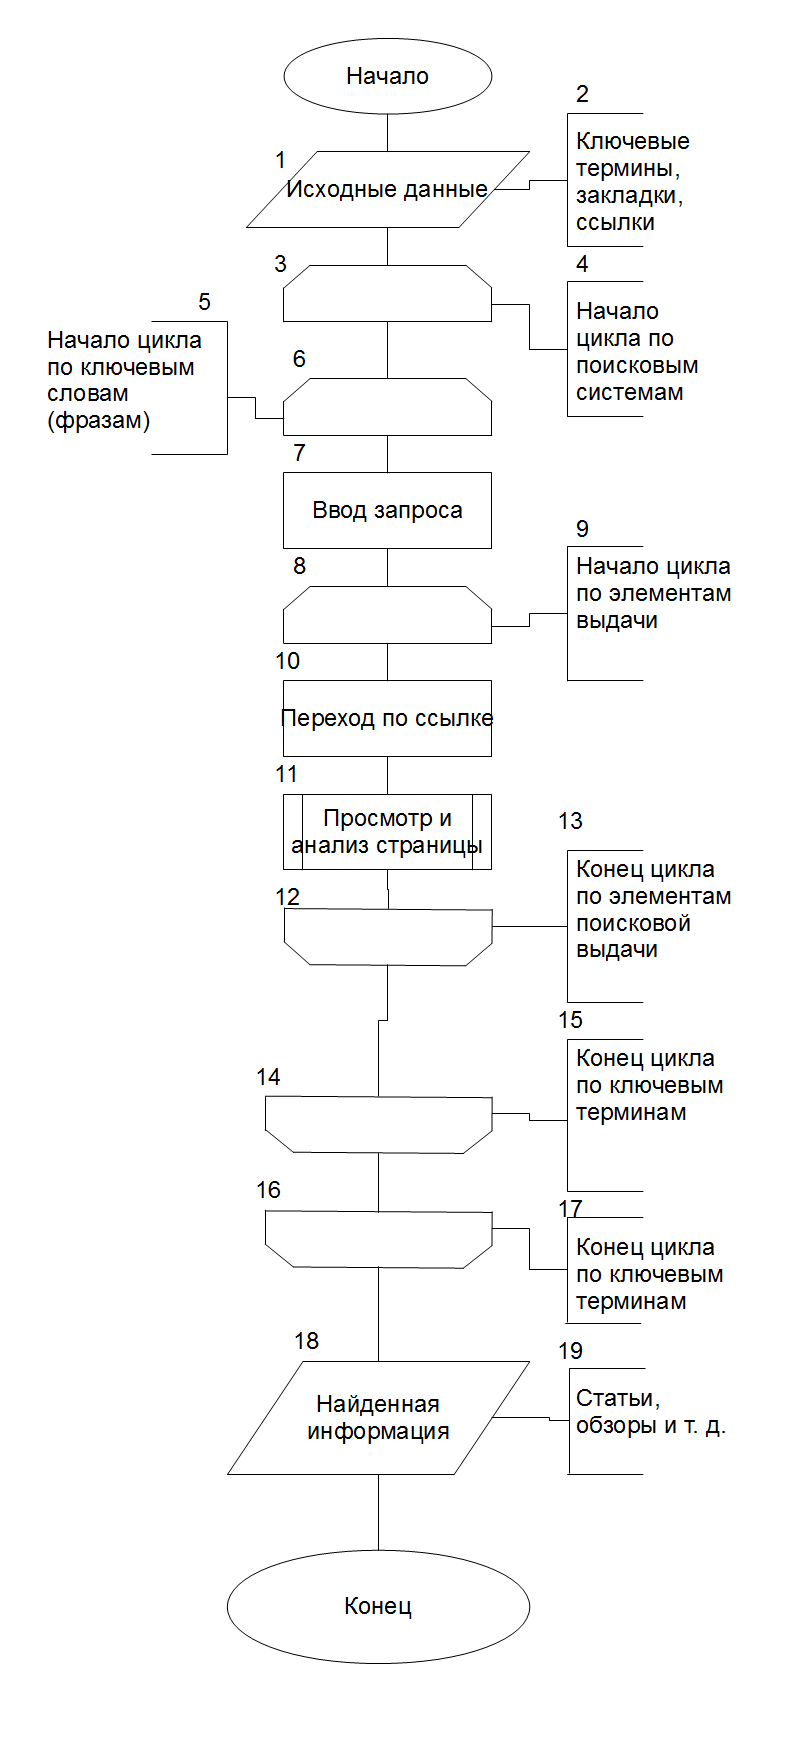
\includegraphics[scale=1.0]{images/searchalg.png}
	\caption{\small Алгоритм поиска информации в Интернете}
	\label{fig:searchalg}
\end{figure}

В приведённом на рисунке \ref{fig:searchalg} алгоритме использовались поисковые машины Google \cite{google}, Bing \cite{bing} и реже Yandex \cite{yandex}.

\subsubsection{Формирование требований к синтаксическому парсеру}
Выделение аналогов среди найденного производилось на основании максимального соответствия следующим предъявляемым к синтаксическим парсерам требованиям:
\begin{list}{\labelitemi}{\leftmargin=1.5cm}
	\item синтаксический парсер должен быть точным (минимальное число ошибок в результирующем дереве разбора, максимально корректное разрешение грамматически неоднозначных ситуаций) --- A;
	\item алгоритм синтаксического анализа должен быть эффективен (минимальная временная сложность алгоритма и сложность алгоритма по памяти, минимальное потребление памяти и процессорной мощности, максимальный потенциально возможный объём анализируемого текста) --- S;
	\item рассматриваемый аналог должен быть совместим с русским языком (минимальная степень специфичности грамматики по отношению к используемому языку, возможность реализовать формальную грамматику для русского языка на основе уже используемой парсером или наличие готовой) --- LS;
	\item входная информация должна быть в минимальной степени формализована (рассматриваемый аналог не должен требовать от входной информации предварительной обработки иными средствами естественноязыкового анализа) --- V.
\end{list}

\subsubsection{Критерии оценки аналогов}
Приведённые выше требования положены в основу четырёх критериев кортежной модели сравнения и оценки аналогов: $O = <A, S, LS, V; R>$,\\
где O --- интегральная оценка аналога, A --- критерий точности разбора, S --- критерий эффективности алгоритма, LS --- критерий простоты локализации грамматики, V --- степень формализации входной информации, R --- матрица связи.

Методы оценки по выделенным критериям следующие:
\begin{list}{\labelitemi}{\leftmargin=1.5cm}
	\item A --- объективная нормированная процентная шкала, за нуль отсчёта взят минимальный показатель;
	\item S --- дискретная шкала, чем выше график производной функции сложности алгоритма, тем ниже оценка;
	\item LS --- дискретная шкала: 0.0 --- локализация грамматики невозможна, 0.25 --- для локализации необходима полная переработка грамматики, 0.50 --- достаточно изменить правила грамматики и провести машинное обучение, 0.75 --- достаточно отредактировать правила грамматики, 1.0 --- существует полноценная формальная грамматика русского языка;
	\item V --- дискретная шкала: 0.0 --- информация в виде метаданных, 0.50 --- информация в виде предварительно размеченного текста, 1.0 --- информация в виде необработанного текста.
\end{list}

Формула расчёта оценки аналога:

O \(= \alpha(A) \cdot A + \alpha(S) \cdot S + \alpha(LS) \cdot LS + \alpha(V) \cdot V\),\\
где 
\(\sum_{i=1}^{n} \alpha_i = 1\), \(\alpha_i\) --- весовой коэффициент соответствующего критерия, n --- количество критериев.

Найдём весовые коэффициенты методом попарного сравнения критериев Томаса Саати \cite{tsaati}. 
Будем использовать шкалу от 1 до 9, где: 
\begin{list}{\labelitemi}{\leftmargin=1.5cm}
  \item 1 --- равенство;
  \item 2 --- промежуточное значение;
  \item 3 --- слабое превосходство;
  \item 4 --- промежуточное значение;
  \item 5 --- сильное превосходство;
  \item 6 --- промежуточное значение;
  \item 7 --- значительное превосходство;
  \item 8 --- промежуточное значение;
  \item 9 --- абсолютное превосходство.
\end{list}
Матрица попарного сравнения представлена в таблице \ref{tab:crit}.

\begin{table}[H]
\centering
\caption{Матрица попарного сравнения критериев}
{\small 
\begin{tabu}to \textwidth{ | X[c] | X[c] | X[c] | X[c] | X[c] | X[c] | X[c] | }
	\hline
          & A   & S   & LS  & V & Среднее & Вес  \\ \hline
	A     & 1   & 3   & 4   & 7 & 3.75    & 0.51 \\
	S     & 1/3 & 1   & 3   & 5 & 2.33    & 0.31 \\
	LS    & 1/4 & 1/3 & 1   & 2 & 0.90    & 0.12 \\
	V     & 1/7 & 1/5 & 1/2 & 1 & 0.43    & 0.06 \\ \hline
	Сумма &     &     &     &   & 7.41    & 1.00 \\
	\hline
\end{tabu}
}
\label{tab:crit}
\end{table}

\subsubsection{Обзор найденных аналогов}

\textbf{Модель биграммной лексической близости} (англ. bigram lexical affinities, BLA) --- описана в \cite{eisner}. Решение о построении синтаксической связи между двумя помеченными словами принимается на основе расстояния между рассматриваемыми словами. Чем выше расстояние между словами в предложении, тем выше вероятность образования корректной связи между ними, поскольку в противном случае образуются члены предложения с множественными связями, каждая из которых независима друг от друга. Таким образом, корректный разбор извлекается из популяции согласно следующему принципу: 
\begin{equation}\begin{split}
	& Pr(words, tags, links) = \prod_{\substack{1 \leq i \leq n}} Pr(tword(i) | tword(i + 1), tword(i + 2)) \\
    & \times\prod_{\substack{1 \leq i, j \leq n}} Pr(L_ij | tword(i), tword(j))
\end{split}\end{equation}

В (1) \(Pr(words, tags, linkgs)\) --- вероятность корректного разбора при заданных словах, метках и связях, \(Pr(L_{ij} | tword(i), tword(j))\) --- вероятность существования связи между помеченными словами i и j, \(Pr(tword(i) | tword(i + 1), tword(i + 2))\) --- вероятность появления i-го слова перед i + 1- и i + 2-м. 

Описанная модель использует контекстно-свободные грамматики и алгоритм парсинга <<снизу вверх>>, позволяя достичь точности парсинга в 75.9\% при алгоритмической сложности \(O(n^3)\).

\textbf{Модель предпочтений выбора} (англ. selectional preferences, SP) --- описана в \cite{eisner}. Модель использует принцип, схожий с принципом работы парсеров, основанных на грамматике связей: каждому слову сопоставлено множество <<идеальных>> родительских и дочерних слов с обеих сторон, вероятность построения связи с которыми для данного слова наиболее высока. Парсер случайным образом (с некоторой вероятностью), строит дизъюнкты для каждого слова, комбинация которых образует один вариант разбора. Из множества вариантов разбора исключаются те, для которых требования построения сразу нескольких дизъюнктов не могут быть выполнены. Это приводит к ренормализации вероятностей для остальных вариантов. Процесс продолжается до выделения единственного оставшегося или наиболее вероятного варианта. Математическое описание модели:
\begin{equation}\begin{split}
	& Pr(words, tags, links) \propto Pr(words, tags, preferences) = \\
	& Pr(words, tags) \cdot Pr(preferences | words, tags) = \\
	& \prod_{\substack{1 \leq i \leq n}} Pr(tword(i) | tword(i + 1), tword(i + 2)) \\
	& \times \prod_{\substack{1 \leq i \leq n}} Pr(preferences(i) | tword(i))
\end{split}\end{equation}

В (2) \(Pr(words, tags, links)\) --- вероятность корректного разбора для текущих слов, меток и связей, \(Pr(words, tags, preferences)\) --- вероятность корректного разбора для текущих слов, меток и предпочтений,\\ \(Pr(tword(i) | tword(i + 1), tword(i + 2))\) --- вероятность появления i-го слова перед i + 1- и i + 2-м, \(Pr(preferences(i) | tword(i))\) --- вероятность выбора i-х предпочтений для i-го слова.

Модель использует контекстно-свободные грамматики, алгоритм парсинга <<снизу вверх>>, достигает точности в 72.8\% при алгоритмической сложности в \(O(n^3 \cdot |G|^2)\).

\textbf{Модель рекурсивной генерации} (англ. recursive generation, RG) --- описана в \cite{eisner}. В отличие от предыдущих двух моделей, которые могут быть отнесены к классу моделей восприятия (comprehension model), данная модель генеративна, то есть, выступает с позиции говорящего, а не слушателя. Каждое слово, поступившее на вход парсера, генерирует с помощью марковских процессов последовательности дочерних пар (tag, word) с левой и с правой стороны. Такой процесс повторяется рекурсивно для каждого сгенерированного слова. Математически данная модель описана следующим образом:
\begin{equation}\begin{split}
	& Pr(words, tags, links) = \\
	& \prod_{\substack{1 \leq i \leq n}} \left( \prod^{\substack{i + \#right-kids(i)}}_{\substack{c = - (1 + \#left-kids(i)), c \neq 0}} Pr(tword(kid_c(i)) | tag(kid_{c - 1}(i)), tword(i)) \right)
\end{split}\end{equation}

В (3) \(Pr(tword(kid_c(i)) | tag(kid_{c - 1}(i)), tword(i))\) --- вероятность генерации c-го дочернего слова с той или иной стороны от i-го родительского слова.

Модель работает на основе контекстно-свободных грамматик и алгоритма парсинга <<снизу-вверх>>, точность разбора до 78.1\% при алгоритмической сложности в \(O(n^5)\).

\textbf{Алгоритм Кокка-Янгера-Касами} (анг. Cocke-Younger-Kasami algorithm, CYK) --- алгоритм парсинга для контекстно-свободных грамматик в нормальной форме Хомского \cite{wiki_cyk}. Один из классических алгоритмов парсинга, он рассматривает каждую допустимую (в соответствии с правилами продукции грамматики) подпоследовательность последовательности слов и устанавливает истинность P(i, j, k), где i и j --- индексы символов последовательности, k --- индекс правила продукции, если связь между i-м и j-м словами может быть построена при помощи k-го правила продукции. Алгоритм последоватльно наращивает расстояние между i и j, пока не достигнет нулевого символа.

Алгоритм CYK также использует принцип CYK, на размеченных последовательностях достигает точности разбора в 66.6\% при алгоритмической сложности \(O(n^3 \cdot |G|)\).

\textbf{Алгоритм диаграммного парсинга Эрли} (анг. Chart Parsing Earley Algorithm, EA) --- алгоритм, описанный в \cite{webbe}. Базируется на алгоритме Кокка-Янгера-Касами (синтаксический парсинг <<снизу вверх>>), но добавляет в исходный алгоритм предсказание следующей относительно текущей позиции во входной строке части речи (предсказание <<сверху вниз>>), таким образом избавляясь от заведомо некорректных дуг дерева разбора. Алгоритм Эрли использует контекстно-независимые грамматики, входная последовательность должна быть предварительно размечена, при этом сложность алгоритма описывается функцией \(O(n^3)\).

\textbf{Парсер на основе грамматики связей} (анг. Link Grammar Parser, LGP) --- метод парсинга, описанный в \cite{sleator}, базируется на свойстве естественных языков, известном как планарность (связи-дуги между словами в высказывании не пересекаются друг с другом). Грамматика связей состоит из множества слов, каждому из которых сопоставлены требования к связям. Связи между словами образуются в том случае, если:
\begin{list}{\labelitemi}{\leftmargin=1.5cm}
	\item связи не пересекаются друг с другом;
	\item все слова последовательности получается связать друг с другом;
	\item связи удовлетворяют требованиям к связям каждого слова в последовательности.
\end{list}

На текущий момент наиболее удачная реализация этого алгоритма выполнена компанией ABBYY, существует корректная (но неполная) грамматика связей для русского языка. Алгоритм работает со сложностью \(O(n^3)\) и достигает точности в 73\%.

\subsubsection{Выбор прототипа}
Выделенные в требованиях характеристики для найденных аналогов были определены и сведены в таблице \ref{tab:obj}.

\begin{table}[H]
\centering
\caption{Результат объективной оценки аналогов по критериям}
{\small 
\begin{tabu}to \textwidth{ | X[c] | X[c] | X[c] | X[c] | X[c] | }
	\hline
    Аналог/Критерий & A    & S                & LS   & V   \\ \hline
	BLA                      & 75.9 & \(O(n^3)\)       & 0.50 & 1.0 \\ \hline
	SP                       & 72.8 & \(O(n^3 \cdot |G|^2)\) & 0.50 & 1.0 \\ \hline
	RG                       & 78.1 & \(O(n^5)\)       & 0.50 & 1.0 \\ \hline
	CYK                      & 66.6 & \(O(n^3 \cdot |G|)\)   & 0.75 & 0.5 \\ \hline
	EA                       & 78.0 & \(O(n^3)\)       & 0.75 & 0.5 \\ \hline
	LGP                      & 73.0 & \(O(n^3)\)       & 1.00 & 1.0 \\ 
	\hline
\end{tabu}
}
\label{tab:obj}
\end{table}

С учётом приведённой ранее системы выставления оценок, объективные показатели были переведены в значения на соответствющих шкалах и нормированы. Результат представлен в таблице \ref{tab:scales}.

\begin{table}[H]
\centering
\caption{Результат нормированной оценки аналогов по шкалам критериев}
{\small 
\begin{tabu}to \textwidth{ | X[c] | X[c] | X[c] | X[c] | X[c] | }
	\hline
    Аналог/Критерий          & A    & S     & LS   & V   \\ \hline
	BLA                      & 0.97 & 1.00  & 0.50 & 1.0 \\ \hline
	SP                       & 0.93 & 0.50  & 0.50 & 1.0 \\ \hline
	RG                       & 1.00 & 0.00  & 0.50 & 1.0 \\ \hline
	CYK                      & 0.85 & 0.75  & 0.75 & 0.5 \\ \hline
	EA                       & 1.00 & 1.00  & 0.75 & 0.5 \\ \hline
	LGP                      & 0.93 & 1.00  & 1.00 & 1.0 \\ 
	\hline
\end{tabu}
}
\label{tab:scales}
\end{table}

Взвешенные оценки, полученные умножением оценки по шкале на соответствующий весовой коэффициент, приведены в таблице \ref{tab:weight}.

\begin{table}[H]
\centering
\caption{Результат оценки аналогов по шкалам критериев}
{\small 
\begin{tabu}to \textwidth{ | X[c] | X[c] | X[c] | X[c] | X[c] | X[c] | }
	\hline
    Аналог/Крит.             & A    & S     & LS   & V    & Сумма \\ \hline
	BLA                      & 0.49 & 0.31  & 0.06 & 0.06 & 0.92  \\ \hline
	SP                       & 0.47 & 0.16  & 0.06 & 0.06 & 0.75  \\ \hline
	RG                       & 0.51 & 0.00  & 0.06 & 0.06 & 0.63  \\ \hline
	CYK                      & 0.43 & 0.23  & 0.09 & 0.03 & 0.78  \\ \hline
	EA                       & 0.51 & 0.31  & 0.09 & 0.03 & 0.94  \\ \hline
	LGP                      & 0.47 & 0.31  & 0.12 & 0.06 & 0.96  \\ 
	\hline
\end{tabu}
}
\label{tab:weight}
\end{table}

Таким образом, по результатам критериальной оценки, получаем в качестве прототипа решение на основе грамматики связей (link grammar parser).

\subsection{Обзор прототипа}
Для проведения критики выбранного прототипа необходимо выделить его структурные блоки и определить связи между ними, то есть построить структурную модель.

\subsubsection{Структурная модель прототипа}
Приведённая на рисунке \ref{fig:prototype_struct} структурная модель прототипа была восстановлена на основе описаний, данных в \cite{sleator}.

\begin{figure}[H]
	\centering
		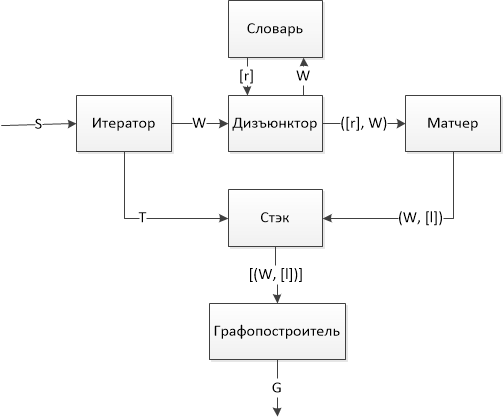
\includegraphics[scale=1.0]{images/initialstructure.png}
	\caption{\small Структурная модель прототипа}
	\label{fig:prototype_struct}
\end{figure}

Функции блоков, изображённых на рисунке \ref{fig:prototype_struct}, следующие:
\begin{list}{\labelitemi}{\leftmargin=1.5cm}
	\item Итератор --- получает на вход исходную последовательность S, разбивает её на отдельные слова W и передаёт в Дизъюнктор; по окончанию последовательности передаёт терминальный символ T в Стэк;
	\item Дизъюнктор --- передаёт полученное от Итератора слово W в Словарь, откуда получает множество правил [r], соответствующих данному слову; на основании этих правил строит дизъюнкты (возможные сочетания для слова W); кортеж, состоящий из слова и множества полученных дьзъюнктов, передаётся в Матчер;
	\item Словарь --- хранит правила продукции грамматики связей, на запрос по слову W возвращает множество правил [r], соответствующих полученному слову W;
	\item Матчер --- сопоставляет полученные дизъюнкты с исходной последовательностью S, определяя их корректность, таким образом строя связи; множество связей [l] для слова W передаётся на Стэк;
	\item Стэк --- аккумулирует пары (слово, связи) до получения терминального символа от Итератора, после чего передаёт данные в графопостроитель;
	\item Графопостроитель --- на основании полученных данных формирует результирующий граф (дерево) синтаксического разбора.
\end{list}

\subsubsection{Критика прототипа и предлагаемое решение}

\textbf{Критика прототипа}. Как видно из модели, приведённой на рисунке \ref{fig:prototype_struct}, прототип использует для своей работы готовые словари, которые либо  генерируются на основе других хранилищ языковой информации (например, база морфологии AOT), либо заранее готовятся вручную для каждого языка. Ручная подготовка словарей экономически невыгодна, требует много времени и внимания для поддержания словарей в корректном и актуальном виде. Генерация же может заметно снизить качество используемых словарей.

\textbf{Предлагаемое решение}. Отказаться от использования словарей, вместо них использовать интерфейс взаимодействия с внешними централизованными хранилищами лингвистической информации в виде готовых онтологий. Это позволит всегда иметь доступ к актуальной и корректной информации и избавит разработчика от необходимости наполнять и поддерживать в обновлённом виде собственные словари.

\subsection{Результаты и выводы по главе 1}

В процессе проведения литературного обзора были достигнуты следующие результаты:
\begin{list}{\labelitemi}{\leftmargin=1.5cm}
	\item выбрана и рассмотрена технология поиска информации по теме;
	\item выбраны критерии для сравнения аналогов и описаны методы постановки оценок по выбранным критериям;
	\item найден ряд аналогов;
	\item найденные аналоги были оценены по степени их соответствия выбранным критериям;
	\item было проведено сравнение аналогов с выделением лучшего решения;
	\item восстановлена структурная модель выбранного прототипа;
	\item с помощью модели прототипа была проведена его критика;
	\item предложено решение по улучшению прототипа.
\end{list}

\textbf{Вывод}: информации, полученной в главе 1 достаточно для перехода к моделированию прототипа и предлагаемого решения.
